\section{S\'ecurit\'e}\label{sec:security}

La sécurité au sein de \acrshort{tor} s'articule autour d'un réseau de noeuds relais comprenant un noeud d'entrée, des noeuds intermédiaires ainsi qu'un noeud de sortie.
Lors de l'initialisation de la connexion entre l'expéditeur et le destinataire, des méthodes cryptographiques avancées (\textit{cfr.}, sec. \ref{subsec:data} "\nameref{subsec:data}") sont utilisées afin de sécuriser non seulement les données transmises mais également leurs canaux de communications.
Le routage en oignon offre l'anonymat en encapsulant les données dans plusieurs couches de chiffrement. 
Chaque nœud dans le circuit ne peut déchiffrer que la couche lui étant assignée, ne révélant jamais l'identité ni de l'expéditeur ni du destinataire.

Les aspects techniques de la sécurité dans \acrshort{tor}, incluant le routage en oignon, la sélection des relais, les protocoles de chiffrement, les mesures défensives et les politiques de confidentialité, contribuent à sa robustesse comme outil d'anonymat en ligne.

La sécurité dans \acrshort{tor} passe par le chiffrement des données ainsi que par la sécurisation des communications.
\begin{enumerate}
  \item \ref{subsec:data} \nameref{subsec:data} chiffrées via cryptographie symétrique et asymétrique
  \item \ref{subsec:comm} \nameref{subsec:comm} sécurisées via poignées de mains \acrfull{dh} et \acrfull{tls}
\end{enumerate}

La Figure \ref{fig:structure-layers} "\nameref{fig:structure-layers}" ci-dessous illustre les différentes couches de sécurité qui se supperposent dans \acrshort{tor}.
Les données étant transmises via des cellules chiffrées via cryptographie symétrique. 
La cryptographie symétrique (\acrshort{sc}) découle d'un processus impliquant la cryptographie asymétrique (\acrshort{ac}) elle-même impliquant les poignées de mains Diffie-Hellman (\acrshort{dh}).
Il est important de noter que les poignées de main \acrshort{dh} ainsi que la \acrshort{ac} n'interviennent qu'au moment de l'établissement du circuit.
Ces dernières utilisent des canaux de communications sécurisés via le protocole \acrshort{tls}.


\begin{figure}[htbp]
  \centering
  \begin{tikzpicture}
    % Main figure
    \node[inner sep=0] (main) {
      \begin{tikzpicture}
        % Layers with hatching
        \begin{scope}
            \clip (0,0) circle (2.2cm);
            \fill[pattern=north west lines] (0,0) circle (2.2cm);
            \fill[white] (0,0) circle (1.3cm);
        \end{scope}
        % Circles and labels
        \draw (0,0) circle (0.7cm) node[align=center] {Cell};
        \draw (0,0) circle (1.3cm) node[yshift=1cm] {SC};
        \draw (0,0) circle (2.2cm) node[yshift=1.7cm] {DH \&\& AC};
        \draw (0,0) circle (2.8cm) node[yshift=2.5cm] {TLS};
      \end{tikzpicture}
    };

    % Legend
    \node[right=10mm of main, inner sep=10pt, draw, rectangle, minimum width=3cm, minimum height=2.5cm, text width=2.8cm] (legend) {
      \raggedright
      \tikz{\fill[pattern=north west lines, pattern color=black] (0,0) rectangle (0.5,0.5);} Initialisation only\\[1ex]
      \tikz{\draw (0,0.25) circle (0.25);} Permanent layers
    };

  \end{tikzpicture}
  \caption{Modélisation des différentes couches de sécurité dans TOR}
  \label{fig:structure-layers}
\end{figure}



\newpage
\subsection{Données}\label{subsec:data}

La sécurité au niveau des données est assurée par une combinaison de cryptographie asymétrique et symétrique pour sécuriser le contenu.

\begin{enumerate}
  \item \ref{subsubsec:cs} \nameref{subsubsec:cs} Utilisée pour déchiffrer les cellules de données transmises.
  \item \ref{subsubsec:ca} \nameref{subsubsec:ca} Utilisée pour l'échange de clés privées.
\end{enumerate}


\subsubsection{Cryptographie symétrique}\label{subsubsec:cs}

La cryptographie symétrique repose sur l'utilisation de clés privées partagées.
Le protocole d'échange de clés \acrlong{dh} permet d'établir la connexion et de générer les clés privées via l'algorithme AES (Advanced Encryption Standard).
Ces clés peuvent être comparées à un cadenas: un code protège le cadenas, quiconque possède le code peut ouvrir ce cadenas, cependant si le code venait à être partagé, cela compromettrait la sécurité apportée par ce cadenas.

La Figure \ref{fig:structure-chiffrement} "\nameref{fig:structure-chiffrement}" ci-dessous illustre la structure de chiffrement d'une cellule au sein du réseau \acrshort{tor}.
La première couche de chiffrement sera déchiffrée par le premier noeud du circuit. 
L'oignon sera ainsi épluché jusqu'à atteindre le dernier noeud et retirer sa dernière couche.
Ce processus permettra ainsi au message d'être transmis au destinataire de manière sécurisée.

\begin{figure}[h!]
  \centering
  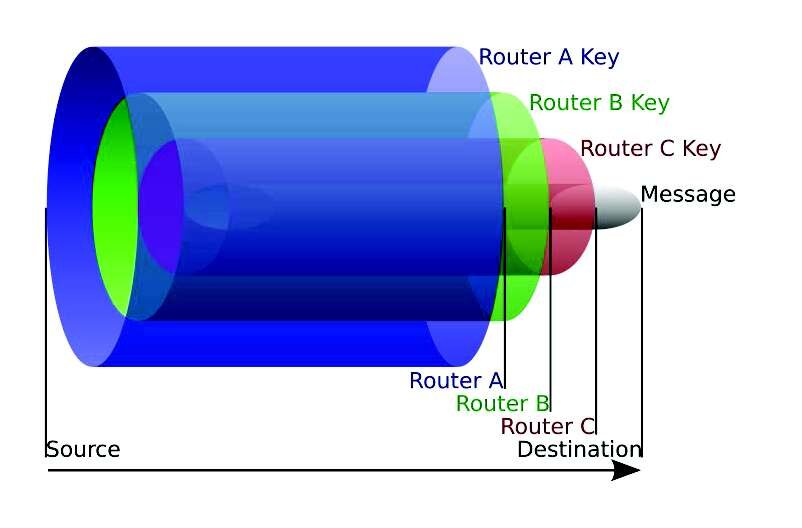
\includegraphics[width=0.7\linewidth]{Images/OR/Layers-of-the-Onion-source.png.jpeg}
  \caption{Structure du chiffrement en couches. \cite[Layers-of-the-Onion-source]{noauthor_layers---onion-sourcepng_nodate}.}
  \label{fig:structure-chiffrement}
\end{figure}

\subsubsection{Cryptographie asymétrique}\label{subsubsec:ca}

La cryptographie asymétrique repose sur l'utilisation d'une paire de clés publique et privée associées.
Ces clés sont mathématiquement liées: dans \acrshort{rsa} il s'agit de la factorisation de grands nombres premiers tandis que dans \acrshort{ecc} il s'agit de logarithmes discrets.

Un message chiffré avec une clé publique ne peut être déchiffré qu'avec la clé privée correspondante: si une personne reçoit un message lui demandant de crier dans un auditoire afin de pouvoir la situer, lorsque celle-ci criera, seule la personne qui le lui aura demandé sera en mesure de déchiffrer le message "Je suis ici", les autres ne disposant tout simplement pas des clés permettant de décoder la situation.
Dans cet exemple, la clé publique est le système de messagerie permettant de cacher le contenu du message aux autres personnes présentes. La clé privée est le contenu du message en lui-même.

\subsubsection{Comparaison cryptographie symétrique et asymétrique}

Le Tableau \ref{tab:tech-crypto} "\nameref{tab:tech-crypto}" ci-dessous permet de mettre en évidence les différences d'usages entre cryptographie symétrique et asymétrique.
D'un côté une cryptographie plus simple à mettre en place et plus adaptée pour le transfert d'importants volumes de données.
De l'autre une cryptographie plus exigeante mais offrant d'avantages de garanties lors du partage de données particulièrement sensibles.
% \begin{table}[htbp]
%     \centering
%     \begin{tabularx}{\textwidth}{
%         >{\raggedright\arraybackslash}p{2cm} 
%         >{\raggedright\arraybackslash}p{6.5cm} 
%         >{\raggedright\arraybackslash}p{6.5cm}}
%         \toprule
%         \rowcolor[HTML]{EFEFEF}
%         \textbf{}               & \textbf{Clés Symétriques}                                                                                                                         & \textbf{Clés Asymétriques} \\
%         \midrule
%         Méthode de chiffrement  & Utilise la même clé pour le chiffrement et le déchiffrement, ce qui rend le processus plus direct mais nécessite une gestion sécurisée de la clé. & Utilise une paire de clés: une publique pour le chiffrement et une privée pour le déchiffrement, facilitant la distribution des clés mais augmentant la complexité. \\
%         \midrule
%         Vitesse                 & Plus rapide due à des opérations moins complexes, idéale pour le chiffrement de grands volumes de données.                                        & Plus lent à cause des opérations cryptographiques plus complexes, adapté pour le chiffrement d'informations sensibles en petites quantités. \\
%         \midrule
%         Gestion des clés        & Nécessite une méthode sécurisée pour partager la clé entre les parties, moins adapté pour les systèmes à grande échelle.                          & La gestion des clés est simplifiée puisque la clé publique peut être distribuée ouvertement, tandis que la clé privée reste secrète. \\
%         \midrule
%         Usage typique           & Favorisé pour le chiffrement des données en transit, comme dans le cas des cellules Tor, où la performance et l'efficacité sont cruciales.        & Utilisé pour les échanges sécurisés initiaux, tels que l'établissement de clés symétriques ou la vérification d'identité, grâce à la sécurité renforcée qu'il offre. \\
%         \bottomrule
%     \end{tabularx}
%     \caption{Comparaison entre clés symétriques et asymétriques}
%     \label{tab:cles-sym-asym}
% \end{table}


% \begin{table}[htbp]
%     \centering
%     \begin{tabularx}{\textwidth}{
%         >{\raggedright\arraybackslash}p{2cm}
%         >{\raggedright\arraybackslash}X
%         >{\raggedright\arraybackslash}X}
%         \toprule
%         \rowcolor[HTML]{EFEFEF}
%         \textbf{}                   & \textbf{Cryptographie Symétrique} & \textbf{Cryptographie Asymétrique} \\
%         \midrule
%         Méthode de chiffrement      & Utilise une seule clé pour chiffrer et déchiffrer les données. & Utilise une paire de clés: une publique pour chiffrer, une privée pour déchiffrer. \\
%         \midrule
%         Algorithmes                 & AES et DES &  \acrshort{rsa} et \acrshort{ecc} \\
%         \midrule
%         Complexité algorithmique    & Opérations basées principalement sur des transformations linéaires simples (par exemple, permutation et substitution). Moins coûteux en termes de ressources de calcul. & Nécessite des opérations mathématiques complexes telles que l'exponentiation modulaire, ce qui entraîne des temps de traitement plus longs et une consommation plus élevée de ressources. \\
%         \midrule
%         Gestion des clés            & La distribution sécurisée des clés pose un défi majeur car chaque paire d'utilisateurs nécessite une clé unique partagée, escaladant le nombre de clés nécessaire de manière exponentielle avec le nombre d'utilisateurs. & Facilite la distribution des clés; seule la clé publique doit être partagée ouvertement, tandis que la clé privée est gardée secrète par chaque utilisateur, simplifiant la gestion des clés même dans de grands réseaux. \\
%         \midrule
%         Utilisation                 & Idéal pour les environnements où la sécurité des lignes de communication des clés peut être garantie. Couramment utilisé pour le chiffrement de données au repos et le chiffrement de masse de données en transit. & Utilisé principalement pour les transactions sécurisées, l'authentification et les signatures numériques où les clés ne doivent pas être échangées via un canal sécurisé, réduisant ainsi le risque d'exposition des clés. \\
%         \midrule
%         Vulnérabilités typiques     & Susceptible à l'analyse des clés si des clés insuffisamment aléatoires ou courtes sont utilisées, ou si la gestion des clés est compromise. & Plus vulnérable aux attaques cryptanalytiques telles que l'attaque par facteurisation pour \acrshort{rsa} ou les attaques sur la logique elliptique pour ECC, en particulier si des paramètres faibles ou mal configurés sont utilisés. \\
%         \bottomrule
%     \end{tabularx}
%     \caption{Comparaison entre la cryptographie symétrique et asymétrique}
%     \label{tab:tech-crypto}
% \end{table}




\begin{table}[htbp]
    \centering
    \begin{tabularx}{\textwidth}{
        >{\raggedright\arraybackslash}p{2cm} 
        >{\raggedright\arraybackslash}X 
        >{\raggedright\arraybackslash}X}
        \toprule
        \rowcolor[HTML]{EFEFEF}
        \textbf{Caractéristique} & \textbf{Cryptographie Symétrique} & \textbf{Cryptographie Asymétrique} \\
        \midrule
        Clés & Unique, partagée & Paire de clés (publique, privée) \\
        \midrule
        Algorithmes & AES, DES & RSA, \acrshort{ecc} \\
        \midrule
        Complexité & Moindre & Élevée \\
        \midrule
        Gestion des clés & Difficile pour de nombreux utilisateurs & Plus simple grâce à la clé publique \\
        \midrule
        Utilisation & Chiffrement de masse, sécurisé si la clé est sûre & Transactions sécurisées, signatures numériques \\
        \midrule
        Vulnérabilités & Analyse des clés, gestion compromise & Attaques cryptanalytiques, paramètres faibles \\
        \bottomrule
    \end{tabularx}
    \caption{Comparaison de la cryptographie symétrique et asymétrique}
    \label{tab:tech-crypto}
\end{table}
    
    



\newpage
\subsection{Communications}\label{subsec:comm}

Il s'agit, ici, d'une combinaison de poignées de mains Diffie-Helman et de connections \acrshort{tls} pour sécuriser les communications.
\begin{enumerate}
  \item \ref{subsubsec:dh} \nameref{subsubsec:dh} Permet de générer des clés privées sans les transmettre directemetn sur le circuit.
  \item \ref{subsubsec:tls} \nameref{subsubsec:tls} Permet de sécuriser les communications entre relais.
\end{enumerate}

\subsubsection{Diffie-Helman}\label{subsubsec:dh}

Les poignées de mains Diffie-Helman permettent aux parties prenantes d'une communication sécurisée par cryptographie asymétrique de générer les clés privées nécessaires à la cryptographie symétrique.

Sur base de paramètres communs, chaque partie génère une clé privée qui lui permettra ensuite de calculer sa clé publique.

Une fois les clés publiques partagées, chaque partie utilise sa propre clé privée ainsi que la clé publique de l'autre partie afin de générer la clé symétrique partagée.

\begin{algorithm}
  \caption{Échange de clés Diffie-Hellman entre Alice et Bob}
  \begin{algorithmic}[1]
    \State Alice et Bob s'accordent sur un nombre premier $p$ et une base $g$.
    \State Alice choisit un nombre secret $a$ et envoie $g^a \mod p$ à Bob.
    \State Bob choisit un nombre secret $b$ et envoie $g^b \mod p$ à Alice.
    \State Alice calcule $(g^b \mod p)^a \mod p$.
    \State Bob calcule $(g^a \mod p)^b \mod p$.
    \State Alice et Bob utilisent ce nombre comme leur clé partagée.
  \end{algorithmic}
\end{algorithm}

\begin{figure}[h!]
  \centering
  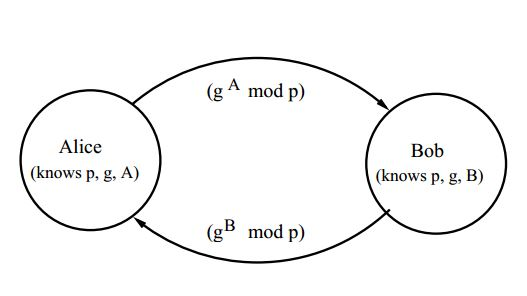
\includegraphics[width=0.7\linewidth]{Images/OR/dh.jpg}
  \caption{Illustration de l'algorithme Diffie-Hellman. \cite[Diffie-Hellman Algorithm.]{spider_diffie-hellman_2024}.}
  \label{fig:dh}
\end{figure}

La motivation principale de l'utilisation de \acrshort{dh} réside dans sa capacité à fournir un secret partagé qui peut ensuite être utilisé pour un chiffrement symétrique robuste, sans que la clé elle-même ne doive être transmise sur le réseau, offrant ainsi une sécurité contre les interceptions.
DH offre également le secret parfait vers l'avant: la compromission des clés privées n'entraîne pas celle des clés de sessions déjà établies.

% Le protocole Diffie-Hellman permet à deux parties de générer une clé secrète partagée sans la transmettre explicitement, en utilisant les étapes suivantes :

% \begin{enumerate}
  %   \item \textbf{Accord sur les paramètres communs :}
  %   Les deux parties s'accordent sur un nombre premier \( p \) et une base \( g \), qui sont publiques.
  
  %   \item \textbf{Génération des clés :}
  %   \begin{itemize}
  %     \item Alice choisit un nombre secret \( a \) et calcule \( A = g^a \mod p \).
  %     \item Bob choisit un nombre secret \( b \) et calcule \( B = g^b \mod p \).
  %     \item Ils échangent \( A \) et \( B \) respectivement.
  %   \end{itemize}
  
  %   \item \textbf{Génération de la clé partagée :}
  %   \begin{itemize}
  %     \item Alice reçoit \( B \) et calcule \( K = B^a \mod p \).
  %     \item Bob reçoit \( A \) et calcule \( K = A^b \mod p \).
  %   \end{itemize}
  % \end{enumerate}
  
  % Cette méthode assure que même si un attaquant peut écouter les échanges de \( A \) et \( B \), il ne peut pas calculer la clé partagée \( K \) sans résoudre le problème difficile du logarithme discret.


\subsubsection{TLS}\label{subsubsec:tls}

\acrfull{tls}, permet d'établir et de sécuriser les communications entre les relais en se basant sur une poignée de mains Diffie-Helman et une méthode de chiffrement (symétrique).

Le protocole \acrshort{tls} utilise donc une combinaison de cryptographie asymétrique pour l'échange de clés et l'authentification ainsi que de cryptographie symétrique pour le chiffrement des données.
